%!TEX root = ..\..\main.tex
\chapter{Deconvolution}
\label{Ch:Deconvolution}

\lhead{Chapter \ref{Ch:Deconvolution}. \emph{Deconvolution}}

%-------------------------------------------------------------------------------
%	Chapter Text
%-------------------------------------------------------------------------------

\section{Introduction}
	In this final chapter, we look at another statistical problem in which we perform an optimization over discrete probability distributions and find that the number of points of support of the maximizing distribution is much smaller than expected. In contrast to Chapter \ref{Ch:Mixtures}, we will take a descriptive and practically minded point of view, rather than the more theory driven previous chapter. This is partly due to the additional complexity of the problem, which prevents many of the tools used on maximum likelihood mixtures from working here. However, this does not stop us from pointing out many similarities between the two problems, and numerical analysis allows us to benefit from the similar phenomenon that occurs.

	The problem is one of \emph{deconvolution}, the recovery of the distribution, $F_X$, or density, $f_X$, of some random variable $X$, from measurements of
	\begin{equation}
		W = X + U
	\end{equation}
	where the measurement error $U$ is independent of $X$. In the case that we know the distribution of $U$, Carroll and Hall \cite{Carroll1988-aj} and Carroll and Stefanski \cite{Stefanski1990-uo} proposed a deconvolution kernel density estimator of $f_X$. If the distribution of $U$ is unknown, then we may hope to estimate it from replicate measurements, $W_{jk} = X_j + U_{jk}$, for $1 \leq k \leq N_j$ and $1 \leq j \leq n$. Delaigle, Hall, and Meister provide an estimator for $f_X$ in this scenario. However, up until Delaigle's and Hall's 2016 paper, ``Methodology for nonparametric deconvolution when the error distribution is unknown,'' \cite{Delaigle2016-la}, there had been no method to estimate the distribution of $X$ when we had no data on the distribution of $U$.

	% [BRIEF SUMMARY OF LITERATURE]

	In this chapter, we focus on the methods introduced in this paper. We will start by summarizing the methods in Section \ref{sec:summary of delaigle hall}. In Section \ref{sec:deconvolution empirical results}, we will empirically demonstrate that these methods produce a similar phenomenon to the one encountered when using maximum likelihood location mixtures, and we will explore how this phenomenon manifests under various conditions. Finally, we point out how we can take advantage of this phenomenon in Section \ref{sec:deconvolution observations and results}.


\section{Summary of Delaigle Hall 2016}
\label{sec:summary of delaigle hall}
	Suppose that we have $n$ observations of
	\begin{align}
		W_j &= X_j + U_j &&j = 1, \dots, n
	\end{align}
	where $X_j$ and $U_j$ are independent and identically distributed as $X$ and $U$ respectively, and $X$ and $U$ are independent. We use $\phi_X$ and $\phi_U$ to denote the characteristics functions of $X$ and $U$, and $F_X$ and $F_U$ for the distributions. We use $f_X$ and $f_U$ for the densities if they exist.

	Suppose also that we do not know any information concerning the distribution of $U$. This is unusual in deconvolution problems; we usually assume that we either know the distribution of $U$, at least up to a scaling factor, or that replicate measurements of the $W_j$s are available for the same $X_j$. 

	\subsection{Assumptions}
	We still make some assumptions about $U$ and its characteristic function, $\phi_U$. These are 
	\begin{assumption}
	\label{assump:phiU real}
		$\phi_U$ is real-valued.
	\end{assumption}
	\begin{assumption}
	\label{assump:phiU non zero}
		For $U$ discrete, $\phi_U$ is non-negative and is zero at at most a countable number of points, and for $U$ continuous, $\phi_U$ is strictly positive on the whole real line.
	\end{assumption}

	Assumption \ref{assump:phiU real} is equivalent to assuming that $F_U$ is symmetric. Assumption \ref{assump:phiU non zero} is a standard assumption in deconvolution problems.

	[WHAT DOES $\phi_U \geq 0$ MEAN FOR $f_U$]

	We also make assumptions on the distribution of $X$. 
	% We write the convolution of distributions $F$ and $G$ as
	% \begin{equation}
	% 	(F \circ G)(x) = \int F(x - u) \intd G(u).
	% \end{equation}
	\begin{assumption}
	\label{assumpt: X not symmetric}
		$F_X$ is not symmetric.
	\end{assumption}
	\begin{assumption}
		\label{assump: X indecomposable}
		It is not possible to decompose $X$ as
		\begin{equation}
			X = Y + Z
		\end{equation}
		for nondegenerate and independent random variables $Y$ and $Z$ with $F_Z$ symmetric.
	\end{assumption}

	We require these assumptions because all we know about $F_U$ is that it is symmetric. So if $F_X$ was also symmetric, we could not distinguish it from $F_U$, and if $X$ is itself made up of a symmetric part $Z$, we could not distinguish $U$ from $Z+U$.


	To form the estimator for $F_X$, we will make use of the \emph{phase function}, which for a random variable $V$, is defined by
	\begin{equation}
		\rho_V = \frac{\phi_V}{|\phi_V|}
	\end{equation}
	on all points where $\phi_V \neq 0$.
	Note that from Assumption \ref{assump:phiU real}, we have that 
	\begin{equation}
	\label{eq: phiU equal mod phiU}
		\phi_U = |\phi_U|
	\end{equation}
	and so $\rho_U = 1$.
	Since $W = X+U$, with $X$ and $U$ independent, we have that
	\begin{align}
		\phi_W = \phi_X \phi_U
	\end{align}
	and so from \eqref{eq: phiU equal mod phiU}, on all points where $\phi_U \neq 0$,
	\begin{align}
		\rho_W = \rho_X.
	\end{align}
	In fact, all random variables of the form $V = X + Z$, where $Z$ is symmetric and independent of $X$, will have phase function $\rho_W$, and the variance of these will satisfy $\var(V) \geq \var(X)$. This motivates the final assumption we make for $X$.

	\begin{assumption}
	\label{assump:X has smallest variance}
		$F_X$ has the uniquely smallest variance out of all distributions with phase function $\rho_X$.
	\end{assumption}

	\subsection{Estimator}
	% The discussion above suggests the following estimator for $F_X$. 
	% we might think to take our estimator of $F_X$ to be the distribution with minimum variance that has phase function equal to an estimator of $\rho_W$ constructed from $W_1, \dots, W_n$. However, there are a few considerations to be made.
	% Firstly, 
	We can estimate $\rho_X = \rho_W$ by
	\begin{equation}
		\hat{\rho}_X = \frac{\hat{\phi}_W}{\left|\hat{\psi}_W\right|^{1/2}}
	\end{equation}
	where
	\begin{equation}
	\label{eq:define hat phi W}
		\hat{\phi}_W(t) = \frac{1}{n}\sum_{j = 1}^n \exp(it W_j)
	\end{equation}
	and 
	\begin{equation}
	\label{eq:define hat psi W}
		\hat{\psi}_W(t) = \frac{1}{n(n-1)} \sum_{k=1}^n \sum_{j \neq k} \exp(it (W_j - W_k)).
	\end{equation}

	Ideally, we would like to choose our estimate for $F_X$ to have phase function $\rho = \hat{\rho}_X$. However, $\hat{\rho}_X(t)$ grows less reliable for large values of $|t|$. So we instead aim to minimise 
	\begin{equation}
		T(F) = \int_{-\infty}^\infty \left| \hat{\phi}_W(t) - \left|\hat{\psi}_W(t)\right|^{1/2} \rho(t) \right|^2 w(t) \intd t,
	\end{equation}
	where $\rho(t)$ is the phase function of the distribution $F$, and $w(t)$ is some non-negative weight function that assigns greater value when $t$ is small. In practise, we perform this minimization over some set of distributions $F$ (for example, discrete distributions with no more than $m$ points of support). Call this set $\mathscr{F}$. Having found
	\begin{equation}
		T_\mathrm{min} = \min_{F \in \mathscr{F}} T(F),
	\end{equation}
	we then choose our estimator to be the distribution $F \in \mathscr{F}$ that has smallest variance, under the constraint that $T(F) = T_\mathrm{min}$.

	\subsection{Numerical Implementation}

	Delaigle and Hall suggest performing this optimization problem by approximating $F_X$ with a discrete distribution on $m$ points. They suggest choosing the location of the probability masses, $\vect{\theta} = (\theta_1, \dots, \theta_m)$, to be fixed and distributed uniformly but randomly along $[\min(W_i), \max(W_i)]$ and letting the probability weights $\vect{p} = (p_1, \dots p_m)$ be the variables over which we find the solution. Denote by $F_{\vect{\theta}, \vect{p}}$ the distribution that places mass $p_j$ at $\theta_j$ for $j = 1,\dots, m$. Its characteristic function is given by
	\begin{equation}
		\phi_{\vect{\theta}, \vect{p}} = \sum_{j = 1}^m p_j \exp(it\theta_j)
	\end{equation}
	and its phase function by
	\begin{equation}
		\rho_{\vect{\theta}, \vect{p}} = \frac{ \sum_{j = 1}^m p_j \exp(it\theta_j)}{\left| \sum_{j = 1}^m p_j \exp(it\theta_j)\right|}.
	\end{equation}
	It has variance
	\begin{equation}
		\var(F_{\vect{\theta}, \vect{p}}) = \sum_{j = 1}^m p_j \theta_j^2 - \left( \sum_{j=1}^m p_j \theta_j \right)^2.
	\end{equation}

	For the weight function, $w(t)$, Delaigle and Hall use the Epanechnikov kernel, rescaled to an interval $[-t^*, t^*]$ where $t^*$ is the smallest $t > 0$ such that 
	\begin{equation}
	\label{eq:define t star}
		\left|\hat{\phi}_W(t)\right| \leq n^{-1/4}.
	\end{equation}
	There is some freedom of choice in the number of points in the approximating discrete distribution but $m = 5\sqrt{n}$ is suggested as reasonable.

	Delaigle and Hall also impose some additional constraints. We desire that 
	\begin{equation}
		\hat{\phi}_U = \frac{\hat{\phi}_W}{\phi_{\vect{\theta}, \hat{\vect{p}}}}
	\end{equation}
	is both symmetric (to be consistent with Assumption \ref{assump:phiU real}) and satisfies $\hat{\phi}_U(t) \leq 1$ (as all characteristic functions must satisfy this). In \cite{Delaigle2016-la}, these are stated as hard constraints, however in practise [CITE CODE OR CORREPONDENCE], these are added via penalty terms to $T(F)$.

	Overall, the final method is as follows.

	\begin{enumerate}
		\item Set $m = 5\sqrt{n}$ and fix $\vect{\theta} = (\theta_1, \dots, \theta_m)$ to be distributed uniformly at random along $[\min(W_i), \max(W_i)]$.
		% \item 
		\item Define $\hat{\phi}_W$ and $\hat{\psi}_W$ as in \eqref{eq:define hat phi W} and \eqref{eq:define hat psi W}.
		\item Define $t^*$ as in \eqref{eq:define t star}.
		\item Define
		\begin{equation}
			T(F_{\vect{\theta}, \vect{p}}) = \int_{-t^*}^{t^*} \left| \hat{\phi}_W(t) - \left|\hat{\psi}_W(t)\right|^{1/2} \frac{ \sum_{j = 1}^m p_j \exp(it\theta_j)}{\left| \sum_{j = 1}^m p_j \exp(it\theta_j)\right|} \right|^2 w(t) \intd t.
		\end{equation}
		where $w(t)$ is the Epanechnikov kernel rescaled to $[-t^*, t^*]$.
		\item
		Calculate
		\begin{equation}
			 \vect{p}' = \argmin_{\vect{p}} \left\{T(F_{\vect{\theta}, \hat{\vect{p}}}) + \mathrm{penalties}(\vect{p}')\right\}
		\end{equation}
		and set
		\begin{align}
			T_\mathrm{min} &= T(F_{\vect{\theta}, \vect{p}'})\\
			\mathrm{penalties}_\mathrm{min} &= \mathrm{penalties}(\vect{p}')
		\end{align}
		\item Calculate
		\begin{equation}
			\hat{\vect{p}} = \argmin \left\{ \sum_{j = 1}^m p_j \theta_j^2 - \left( \sum_{j=1}^m p_j \theta_j \right)^2 \right\}
		\end{equation}
		subject to
		\begin{equation}
			T(F_{\vect{\theta}, \vect{p}}) \leq T_\mathrm{min}
		\end{equation}
		and 
		\begin{equation}
			\mathrm{penalties} \leq \mathrm{penalties}_\mathrm{min}
		\end{equation}
		\item The final estimator for $F_X$ is $\hat{F}_X = F_{\vect{\theta}, \hat{\vect{p}}}$.
	\end{enumerate}
	[BE MORE PRECISE ABOUT PENALTIES?]


	\subsection{Converting to continuous distribution}

	If $X$ is continuous, then we will often want to use $\hat{F}_X = F_{\vect{\theta}, \vect{p}}$ to create an estimate of the density, $f_X$. Perhaps the most obvious solution is to use
	\begin{equation}
		\hat{f}_X(x) = \sum_{j=1}^m p_j K_h(x - \theta_j)
	\end{equation}
	where $K_h(x)$ is a kernel with some bandwidth $h > 0$. This is exactly equivalent to 
	\begin{equation}
		\hat{f}_X(x) = \frac{1}{2\pi}\int_{-\infty}^{\infty} \euler^{-itx} \phi_{\vect{\theta}, \vect{p}} \phi_K(ht) \intd t
	\end{equation}
	where $\phi_K$ is the Fourier transform of $K_1(x)$. However, since we only used $t \in [-t^*, t^*]$ when constructing $\phi_{\vect{\theta}, \vect{p}}$, it is reasonable to assume that $\phi_{\vect{\theta}, \vect{p}}$ is less reliable for $t$ outside this range. This motivates replacing $\phi_{\vect{\theta}, \vect{p}}$ with
	\begin{equation}
		\tilde{\phi} = 
		\begin{cases}
			\phi_{\vect{\theta}, \vect{p}}, & t \in [-t^*, t^*],\\
			r(t), & \text{otherwise},
		\end{cases}
	\end{equation}
	where $r(t)$ is some ridge function. Delaigle and Hall suggest following \cite{Delaigle2008-hl} and using
	\begin{equation}
		r = \hat{\phi}_W / \hat{\phi}_{U,P}
	\end{equation}
	where $\hat{\phi}_{U,P}$ is the characteristic function of a Laplace distribution with variance equal to an estimator of the variance of $U$. They also suggest choosing the bandwidth, $h$, using the two-stage plug-in bandwidth of Delaigle and Gijbels \cite{Delaigle2002-pa} \cite{Delaigle2004-fy}.

	We wish to remark here that the conversion from the discrete $F_{\vect{\theta}, \vect{p}}$ to the continuous $\hat{f}_X(x)$ has no effect on the phenomenon of interest in this chapter. We are interested only in the discrete distribution $F_{\vect{\theta}, \vect{p}}$. However, we have included this section for completeness.



	% From here to the end of Section \ref{ssec:KernelSmoothing} is a summary of \cite{Delaigle2016-la}.
	% We want to find the distribution of a random variable $X$ but only measure 
	% $$W = X + U$$
	% where $U$ is symmetric (and hence $\phi_U(t)$ is real-valued and even). We also additionally require that $\phi_U(t) \geq 0$. We write
	% $$\rho_X = \frac{\phi_X}{|\phi_X|}$$
	% for the phase function of $X$. Then 
	% \begin{align*}
	% \phi_W &= \phi_X \phi_U	&&\text{as $X$ and $U$ are independent,}\\
	% \frac{\phi_W}{|\phi_W|} &= \frac{\phi_X}{|\phi_X|}\frac{\phi_U}{|\phi_U|},\\
	% \rho_W &= \rho_X	&&\text{as $\phi_U$ is real and non-negative.}
	% \end{align*}

	% Given a probability distribution, there are an infinite number of other distributions that have the same phase function. We make the choice that out of all the distributions with phase function $\rho_W$, we choose the one that has smallest variance. Hence, we want to find a distribution $F_Y$ that minimizes $\var(Y)$ such that
	% $$\rho_Y = \rho_W.$$

	% \subsection{Optimization problem}
	% 	\label{ssec:optimizationproblem}
	% 	Ideally, we would like to minimize the variance of $Y$ under the constraint that $\rho_Y = \rho_W$. However, we can't do this since we only estimate $\rho_W(t)$ from a random sample of size $n$ and this estimate is bad for large $|t|$. So we instead choose a $Y_0$ to minimize 
	% 	\begin{equation}
	% 	T(Y) = \int_{-\infty}^{\infty} \Big| \hat{\phi}_W(t) - |\hat{\phi}_W(t)| \rho_Y(t) \Big|^2 w(t) \intd t
	% 	\end{equation}\label{eq:T(Y)}
	% 	where $w(t)$ is some suitably chosen weight function and $\hat{\phi}_W(t)$ is our empirical estimate for $\phi_W(t)$. We then search for $Y$ which minimizes $\var(Y)$ subject to $T(Y) \leq T(Y_0)$.

	% 	We restrict our search to $Y$ discrete with point masses $p_j$ at locations $x_j$ for $j = 1,2,\dots,m$. We place our $x_j$ uniformly at random along the interval $[\min W, \max W]$ and choose the $p_j$ to solve the optimization problem described above. Numerical investigations indicate that $m = 5 \sqrt{n}$ is a reasonable choice.

	% \subsection{Kernel Smoothing}
	% 	\label{ssec:KernelSmoothing}
	% 	Once we have our discrete distribution $Y$ we can create a continuous density approximation using
	% 	\begin{equation}
	% 	\hat{f}_Y(x) = \frac{1}{2\pi} \int e^{-itx} \phi_Y(t) \phi_K(ht)  \intd t
	% 	\label{eq:f_Y(x)integral}
	% 	\end{equation}
	% 	where $K$ is some kernel with bandwidth $h$. This is exactly equivalent to
	% 	\begin{equation}
	% 	\hat{f}_Y(x) = \sum_{j=1}^m p_j K_h(x - x_j).
	% 	\label{eq:f_Y(x)sum}
	% 	\end{equation}

	% 	However, we can get a better result by using \eqref{eq:f_Y(x)integral} and replacing $\phi_Y(t)$ with an appropriate ridge function for $t \geq t^*$.
		%Ridging stuff
		%Choice of bandwidth
		%Integral considerations (stuff I did about how to integrate this thing)

\section{Empirical Results}
\label{sec:deconvolution empirical results}
% \section{Examples and Relation to Mixture Phenomenon}

	\begin{figure}
		\centering
		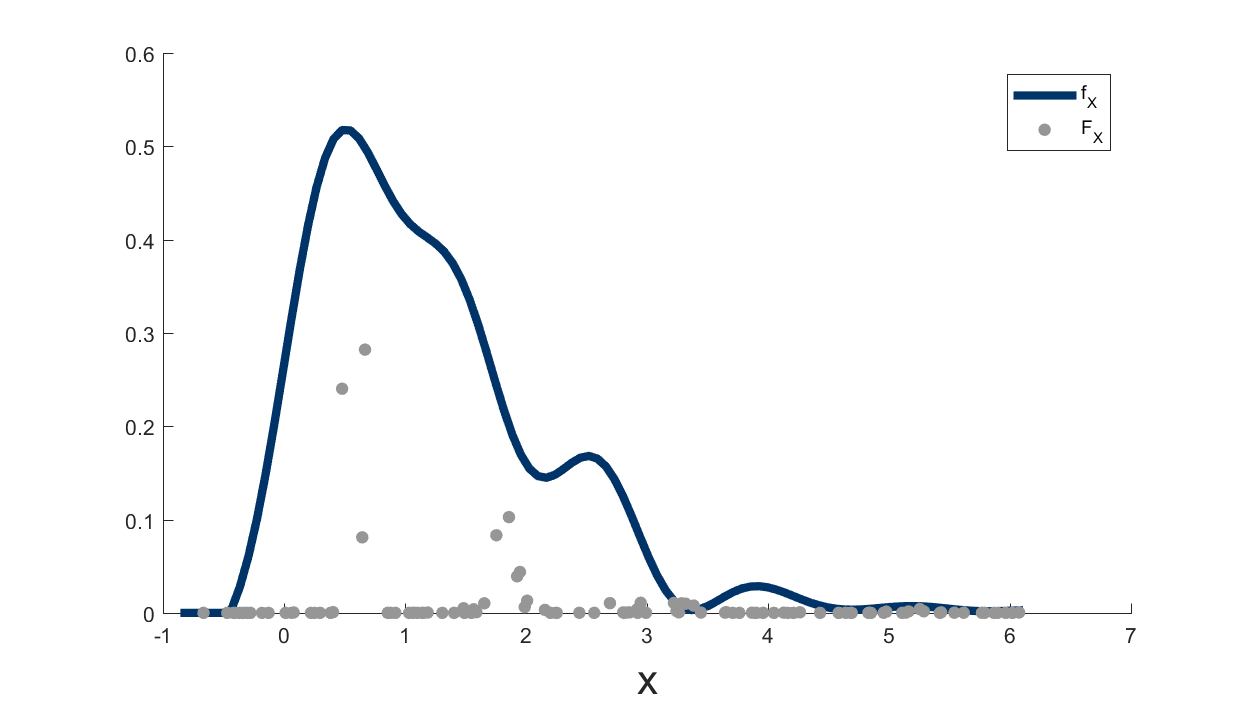
\includegraphics[width = \textwidth]{Figures/Deconvolution/fixed_masses_example.png}
		\caption{hello}
		\label{fig:fixed masses example}
	\end{figure}

	\begin{figure}
		\centering
		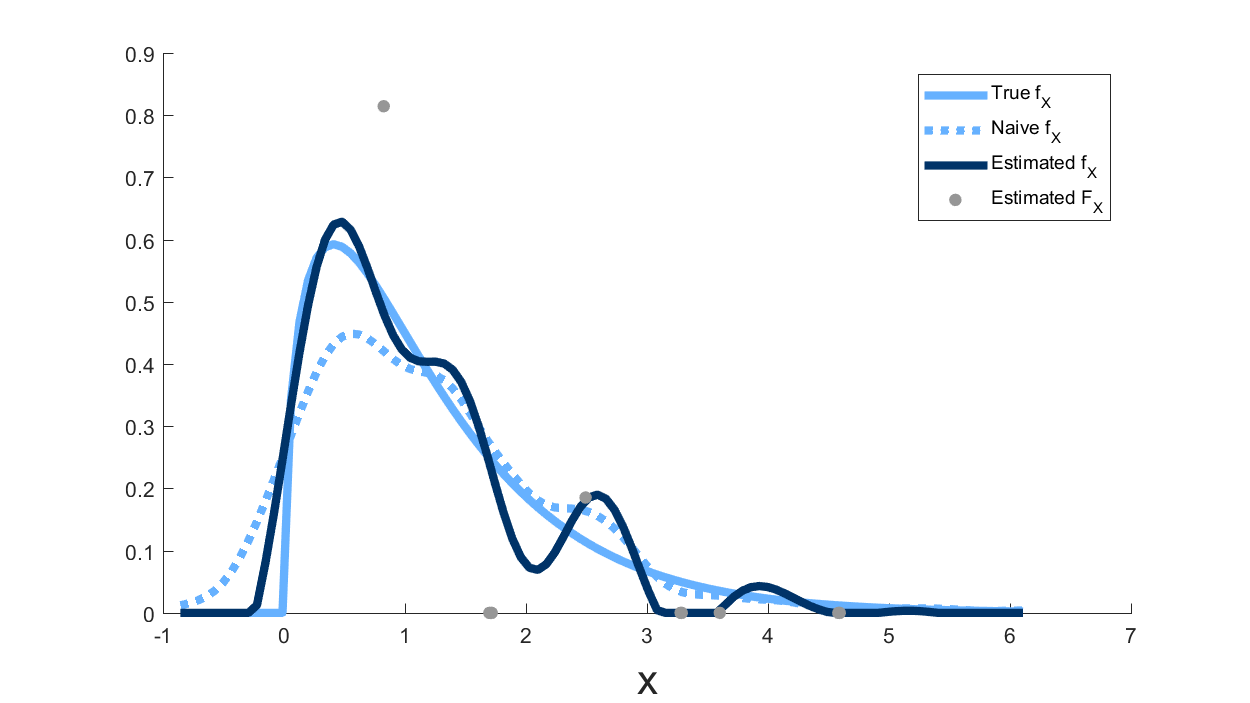
\includegraphics[width = \textwidth]{Figures/Deconvolution/moving_masses_example.png}
		\caption{hello}
		\label{fig:moving masses example}
	\end{figure}

\section{General Observations and Results}
\label{sec:deconvolution observations and results}
	
	\subsection{Results concerning phase functions}
	\begin{theorem}
		Let $F_X$ and $F_Y$ be two distributions, and let
		\begin{align}
			F_Z &= (1 - \lambda) F_X + \lambda F_Y && \lambda \in [0,1]
		\end{align}
		be a convex combination of these distributions. If $\rho_X = \rho_Y$, then 
		\begin{equation}
			\rho_Z = \rho_X = \rho_Y.
		\end{equation}
	\end{theorem}
	\begin{proof}
		Write $\phi_X$ and $\phi_Y$ for the characteristic functions of $X$ and $Y$. These are complex valued functions which we can write in the form
		\begin{align}
			\phi_X &= r_X(t) \euler^{i\theta_X(t)},\\
			\phi_Y &= r_Y(t) \euler^{i\theta_Y(t)},
		\end{align}
		where $r_X(t), r_Y(t)$ take values on $[0, 1]$ and where
		\begin{align}
			\rho_X &= \euler^{i\theta_X(t)},\\
			\rho_Y &= \euler^{i\theta_Y(t)}.
		\end{align}
		The characteristic function of $F_Z$ is 
		\begin{align}
			\phi_Z &= \int \euler^{itx} \intd \left[(1 - \lambda)F_X(x) + \lambda F_Y(x)\right]\\
			&= (1 - \lambda)\phi_X + \lambda \phi_Y\\
			&= (1 - \lambda) r_X(t) \rho_X + \lambda r_Y(t) \rho_Y.
		\end{align}

		If $\rho_X = \rho_Y$ then
		\begin{equation}
			\phi_Z = \left((1 - \lambda)r_X(t) + \lambda r_Y(t)\right) \rho_X
		\end{equation}
		and so 
		\begin{equation}
			\rho_Z = \rho_X = \rho_Y.
		\end{equation}
	\end{proof}


	% TESTING
	% \begin{proof}
	% 	\begin{align}
	% 		|\rho_Z - \rho_W| &= \left| \frac{(1 - \lambda)\phi_X + \lambda \phi_Y}{|(1 - \lambda)\phi_X + \lambda \phi_Y|} - \rho_W \right|\\
	% 		&= \left| \frac{(1 - \lambda)\phi_X + \lambda \phi_Y - |(1 - \lambda)\phi_X + \lambda \phi_Y| \rho_W}{|(1 - \lambda)\phi_X + \lambda \phi_Y|}\right|
	% 	\end{align}

	% 	\begin{align}
	% 		\phi_Z &= (1 - \lambda) r_X \rho_X + \lambda r_Y \rho_Y\\
	% 		|\phi_Z| &\leq (1 - \lambda) r_X + \lambda r_Y\\
	% 		\phi_Z &= (1 - \lambda) r_X \rho_X + \lambda r_Y \rho_X + \lambda r_Y (\rho_Y - \rho_X)\\
	% 	\end{align}
	% \end{proof}

\subsection{A particular class of optimization problem}
		"The results follow from this general theorem which seems obvious."

		\begin{theorem}
			\label{thm:solution in interior}
			Let $(E_m)_{m=1}^\infty$ be a sequence of appropriately defined sets and let
			$(g_m)_{m=1}^\infty, g_m: E_m \mapsto \mathbb{R}$ be a sequence of
			functions that satisfy the following properties
			\begin{enumerate}
				\item $\forall \vect{x} \in \partial E_m, \exists n < m, \vect{y} \in E_n$ such that
				$g_m(\vect{x}) \leq g_n(\vect{y})$.
				\label{prop:one}
				\item $\exists m_0, \vect{x}_0 \in E_{m_0}$ such that $\forall m, \vect{x} \in 
				E_m$, $g_m(\vect{x}) \leq g_{m_0}(\vect{x}_0)$.
			\end{enumerate}
			Then $\exists m_*, \vect{x}_* \in E_{m_*} \setminus \partial E_{m_*}$ such
			that $\forall m, \vect{x} \in E_m$, $g_m(\vect{x}) \leq g_{m_*}(\vect{x}_*)$.
		\end{theorem}
		\begin{proof}
			The proof is simple. If $\vect{x}_0 \notin \partial E_{m_0}$ then we are done.
			Otherwise, by property \ref{prop:one} we can find a $n$ and $\vect{y} \in 
			E_n$ such that $g_n(y) = g_{m_0}(\vect{x}_0)$. If $\vect{y} \notin \partial 
			E_n$ then we are done, otherwise we repeat the process until we find a $m, 
			\vect{x}$ pair with $\vect{x} \notin \partial E_m$. %Note that property 
			% \ref{prop:one} implies that $\partial E_1 = \emptyset$ and so this process
			% must end.
		\end{proof}

\section{R Package}